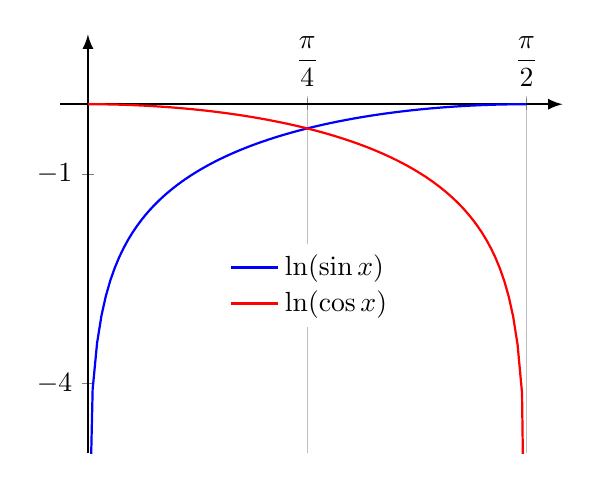
\begin{tikzpicture}
\begin{axis}[
    width=8cm,
    unit vector ratio*=1 0.5 1,
    xlabel={},
    ylabel={},
    xmin=-0.1, xmax=1.7,
    ymin=-5, ymax=1,
    xtick={0,0.7854,1.5708}, 
    xticklabel style={above=5pt},
    xticklabels={$0$,$\displaystyle \frac{\pi}{4}$,$\displaystyle \frac{\pi}{2}$},
    ytick={-1,-4},
    yticklabels={$-1$, $-4$},
    ticklabel style={fill=white},
    xmajorgrids,
    axis lines=middle,
    axis line style=thick,
    axis line style={-latex},
    samples=100,
    % legend pos=south center,
    legend style={
            at={(0.5,0.3)},
            anchor=south, 
            % at={(1.5708,0.5)},
            % anchor=north,
            legend cell align=left,
            draw=none % Unterdrücke Box
        },
]

\addplot[blue,thick, domain=0.001:1.5708] {ln(sin(deg(x)))};
\addplot[red,thick, domain=0.001:1.5708] {ln(cos(deg(x)))};
\legend{$\ln(\sin x)$, $\ln(\cos x)$}

\end{axis}
\end{tikzpicture}
